% !TeX program = pdflatex
% !TeX root = FCLoopValidTopologyQ.tex

\documentclass[../FeynCalcManual.tex]{subfiles}
\begin{document}
\hypertarget{fcloopvalidtopologyq}{
\section{FCLoopValidTopologyQ}\label{fcloopvalidtopologyq}\index{FCLoopValidTopologyQ}}

\texttt{FCLoopValidTopologyQ[\allowbreak{}topo]} returns \texttt{True}
if \texttt{topo} is a valid \texttt{FCTopology} object or a list
thereof.

\subsection{See also}

\hyperlink{toc}{Overview}, \hyperlink{fctopology}{FCTopology}.

\subsection{Examples}

This is a valid topology: it has an id, a list of propagators, a list of
loop and external momenta, a list of possible substitutions for
kinematic invariants and an empty list reserved for future applications

\begin{Shaded}
\begin{Highlighting}[]
\OperatorTok{\{}\NormalTok{FAD}\OperatorTok{[}\NormalTok{p1}\OperatorTok{],}\NormalTok{ FAD}\OperatorTok{[}\NormalTok{p2}\OperatorTok{],}\NormalTok{ FAD}\OperatorTok{[}\NormalTok{p3}\OperatorTok{],}\NormalTok{ FAD}\OperatorTok{[}\FunctionTok{Q} \SpecialCharTok{{-}}\NormalTok{ p1 }\SpecialCharTok{{-}}\NormalTok{ p2 }\SpecialCharTok{{-}}\NormalTok{ p3}\OperatorTok{],}\NormalTok{ FAD}\OperatorTok{[}\FunctionTok{Q} \SpecialCharTok{{-}}\NormalTok{ p1 }\SpecialCharTok{{-}}\NormalTok{ p2}\OperatorTok{],}\NormalTok{ FAD}\OperatorTok{[}\FunctionTok{Q} \SpecialCharTok{{-}}\NormalTok{ p1}\OperatorTok{],}\NormalTok{ FAD}\OperatorTok{[}\FunctionTok{Q} \SpecialCharTok{{-}}\NormalTok{ p2}\OperatorTok{],}\NormalTok{ FAD}\OperatorTok{[}\NormalTok{p1 }\SpecialCharTok{+}\NormalTok{ p3}\OperatorTok{]\}}
\end{Highlighting}
\end{Shaded}

\begin{dmath*}\breakingcomma
\left\{\frac{1}{\text{p1}^2},\frac{1}{\text{p2}^2},\frac{1}{\text{p3}^2},\frac{1}{(-\text{p1}-\text{p2}-\text{p3}+Q)^2},\frac{1}{(-\text{p1}-\text{p2}+Q)^2},\frac{1}{(Q-\text{p1})^2},\frac{1}{(Q-\text{p2})^2},\frac{1}{(\text{p1}+\text{p3})^2}\right\}
\end{dmath*}

\begin{Shaded}
\begin{Highlighting}[]
\NormalTok{topo }\ExtensionTok{=}\NormalTok{ FCTopology}\OperatorTok{[}\NormalTok{topo1}\OperatorTok{,} \OperatorTok{\{}\NormalTok{FAD}\OperatorTok{[}\NormalTok{p1}\OperatorTok{],}\NormalTok{ FAD}\OperatorTok{[}\NormalTok{p2}\OperatorTok{],}\NormalTok{ FAD}\OperatorTok{[}\NormalTok{p3}\OperatorTok{],}\NormalTok{ FAD}\OperatorTok{[}\FunctionTok{Q} \SpecialCharTok{{-}}\NormalTok{ p1 }\SpecialCharTok{{-}}\NormalTok{ p2 }\SpecialCharTok{{-}}\NormalTok{ p3}\OperatorTok{],}\NormalTok{ FAD}\OperatorTok{[}\FunctionTok{Q} \SpecialCharTok{{-}}\NormalTok{ p1 }\SpecialCharTok{{-}}\NormalTok{ p2}\OperatorTok{],} 
    
\NormalTok{    FAD}\OperatorTok{[}\FunctionTok{Q} \SpecialCharTok{{-}}\NormalTok{ p1}\OperatorTok{],}\NormalTok{ FAD}\OperatorTok{[}\FunctionTok{Q} \SpecialCharTok{{-}}\NormalTok{ p2}\OperatorTok{],}\NormalTok{ FAD}\OperatorTok{[}\NormalTok{p1 }\SpecialCharTok{+}\NormalTok{ p3}\OperatorTok{]\},} \OperatorTok{\{}\NormalTok{p1}\OperatorTok{,}\NormalTok{ p2}\OperatorTok{,}\NormalTok{ p3}\OperatorTok{\},} \OperatorTok{\{}\FunctionTok{Q}\OperatorTok{\},} \OperatorTok{\{\},} \OperatorTok{\{\}]}
\end{Highlighting}
\end{Shaded}

\begin{dmath*}\breakingcomma
\text{FCTopology}\left(\text{topo1},\left\{\frac{1}{\text{p1}^2},\frac{1}{\text{p2}^2},\frac{1}{\text{p3}^2},\frac{1}{(-\text{p1}-\text{p2}-\text{p3}+Q)^2},\frac{1}{(-\text{p1}-\text{p2}+Q)^2},\frac{1}{(Q-\text{p1})^2},\frac{1}{(Q-\text{p2})^2},\frac{1}{(\text{p1}+\text{p3})^2}\right\},\{\text{p1},\text{p2},\text{p3}\},\{Q\},\{\},\{\}\right)
\end{dmath*}

\begin{Shaded}
\begin{Highlighting}[]
\NormalTok{FCLoopValidTopologyQ}\OperatorTok{[}\NormalTok{topo}\OperatorTok{]}
\end{Highlighting}
\end{Shaded}

\begin{dmath*}\breakingcomma
\text{True}
\end{dmath*}

This topology is missing information about loop and external momenta

\begin{Shaded}
\begin{Highlighting}[]
\NormalTok{topoWrong }\ExtensionTok{=}\NormalTok{ FCTopology}\OperatorTok{[}\NormalTok{topo1}\OperatorTok{,} \OperatorTok{\{}\NormalTok{FAD}\OperatorTok{[}\NormalTok{p1}\OperatorTok{],}\NormalTok{ FAD}\OperatorTok{[}\NormalTok{p2}\OperatorTok{],}\NormalTok{ FAD}\OperatorTok{[}\FunctionTok{Q} \SpecialCharTok{{-}}\NormalTok{ p1 }\SpecialCharTok{{-}}\NormalTok{ p2 }\SpecialCharTok{{-}}\NormalTok{ p3}\OperatorTok{],}\NormalTok{ FAD}\OperatorTok{[}\FunctionTok{Q} \SpecialCharTok{{-}}\NormalTok{ p1 }\SpecialCharTok{{-}}\NormalTok{ p2}\OperatorTok{],} 
    
\NormalTok{    FAD}\OperatorTok{[}\FunctionTok{Q} \SpecialCharTok{{-}}\NormalTok{ p1}\OperatorTok{],}\NormalTok{ FAD}\OperatorTok{[}\NormalTok{p1 }\SpecialCharTok{+}\NormalTok{ p3}\OperatorTok{]\},} \OperatorTok{\{\},} \OperatorTok{\{\}]}
\end{Highlighting}
\end{Shaded}

\begin{dmath*}\breakingcomma
\text{FCTopology}\left(\text{topo1},\left\{\frac{1}{\text{p1}^2},\frac{1}{\text{p2}^2},\frac{1}{(-\text{p1}-\text{p2}-\text{p3}+Q)^2},\frac{1}{(-\text{p1}-\text{p2}+Q)^2},\frac{1}{(Q-\text{p1})^2},\frac{1}{(\text{p1}+\text{p3})^2}\right\},\{\},\{\}\right)
\end{dmath*}

\begin{Shaded}
\begin{Highlighting}[]
\NormalTok{FCLoopValidTopologyQ}\OperatorTok{[}\NormalTok{topoWrong}\OperatorTok{]}
\end{Highlighting}
\end{Shaded}

\FloatBarrier
\begin{figure}[!ht]
\centering
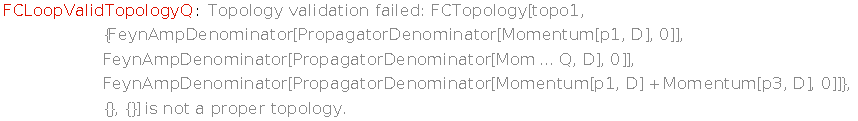
\includegraphics[width=0.6\linewidth]{img/074ejzubvewb2.pdf}
\end{figure}
\FloatBarrier

\begin{dmath*}\breakingcomma
\text{False}
\end{dmath*}
\end{document}
